\documentclass[tikz]{standalone}
\usepackage{tikz}
\usetikzlibrary{patterns,arrows,calc,decorations.pathmorphing}
\usepackage{amsmath}
\usepackage{amsfonts}
\usepackage{amssymb}
\usepackage{enumitem}
% Modified \textcircled macro
\renewcommand*\textcircled[1]{\tikz[baseline=(char.base)]{
  \node [shape=circle,draw,inner sep=1pt] (char) {#1};}}
%\renewcommand*\boxcenter{1.5}

%\newcommand{\brussel}[3]% [position, rotation], content
%{   \begin{tikzpicture}[overlay]
%	\draw [rotate=#3] (#1, #2) rectangle (#1+0.01, #2+0.02);  
% \draw [rotate= #3, blue, very thin] (#1-0.02,#2+0.02) arc (60:120:0.1);	
%\end{tikzpicture}
%}

\begin{document}
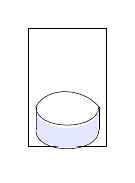
\begin{tikzpicture}
   	\draw [very thin] (0, 0) rectangle (1, 1.5);
	\newcommand*{\tankxa}{0.1}	
	\newcommand*{\tankya}{0.2}	
	\newcommand*{\tankxb}{0.9}	
	\newcommand*{\tankyb}{0.2}	
	\newcommand*{\tankxc}{0.1}	
	\newcommand*{\tankyc}{0.5}	
	\newcommand*{\tankxd}{0.9}	
	\newcommand*{\tankyd}{0.5}	
	\newcommand*{\tankradius}{1}	
	
%
%	
 \draw [very thin] (\tankxa,\tankya) to[out=-90,in=-90] (\tankxb,\tankyb);
  \draw [very thin] (\tankxc,\tankyc) to[out=-90,in=-90] (\tankxd,\tankyd);
  \draw [very thin] (\tankxc,\tankyc) to[out=60,in=130] (\tankxd,\tankyd);
 \draw [very thin] (\tankxa,\tankya) to (\tankxc,\tankyc);
  \draw [very thin] (\tankxb,\tankyb) to (\tankxd,\tankyd);
\fill[fill=blue!10]
   (\tankxa + 0.01,\tankya+0.01) to[out=-90,in=-90] (\tankxb - 0.01,\tankyb+ 0.01) -- (\tankxd -0.01,\tankyd -0.04) to[out=-90,in=-90] (\tankxc + 0.01,\tankyc - 0.04) -- cycle ;

\newcommand*{\pmonecentx}{}

% \draw [very thin, \aracolor](\topantennaposx - \antennasep,\antennacenter + \antennamiddle) to[out=180,in=180] (\topantennaposx - \antennasep, \antennacenter + \antennamiddle + \antennahalfsize);
%	\newcommand*{\containerxa}{1.25}
%	\newcommand*{\containerxb}{1.75}
%	\newcommand*{\containerya}{0.1}
%	\newcommand*{\containeryb}{0.9}
%
%   	\draw (\containerxa, \containerya) rectangle (\containerxb, \containeryb);   
%
%
%	\newcommand*{\brucolor}{blue}		
%	\newcommand*{\bruposxfirst}{1.35}
%	\newcommand*{\bruposxsec}{1.64}
%	\newcommand*{\bruposxthird}{1.36}
%	\newcommand*{\bruposyfirst}{0.75}
%	\newcommand*{\bruposysec}{0.75}
%	\newcommand*{\bruposythird}{0.55}
%	\newcommand*{\brurotfirst}{45}
%	\newcommand*{\brurotsec}{-45}
%	\newcommand*{\brurotthird}{135}
%	\newcommand*{\brusquaresizex}{0.01}
%	\newcommand*{\brusquaresizey}{0.02}
%
%	\draw [rotate around={\brurotfirst:(\bruposxfirst,\bruposyfirst)},very thin, blue]  (\bruposxfirst, \bruposyfirst) rectangle (\bruposxfirst+\brusquaresizex, \bruposyfirst+\brusquaresizey);  
%	\draw [rotate around={\brurotfirst:(\bruposxfirst,\bruposyfirst)},very thin, blue] (\bruposxfirst -0.06,\bruposyfirst+0.05) arc (135:45:0.1);
%
%	\draw [rotate around={\brurotsec:(\bruposxsec,\bruposysec)},very thin, blue]  (\bruposxsec, \bruposysec) rectangle (\bruposxsec+\brusquaresizex, \bruposysec+\brusquaresizey);  
%	\draw [rotate around={\brurotsec:(\bruposxsec,\bruposysec)},very thin, blue] (\bruposxsec -0.06,\bruposysec+0.05) arc (135:45:0.1);
%
%	\draw [rotate around={\brurotthird:(\bruposxthird,\bruposythird)},very thin, blue]  (\bruposxthird, \bruposythird) rectangle (\bruposxthird+\brusquaresizex, \bruposythird+\brusquaresizey);  
%	\draw [rotate around={\brurotthird:(\bruposxthird,\bruposythird)},very thin, blue] (\bruposxthird -0.06,\bruposythird+0.05) arc (135:45:0.1);
%
%\newcommand*{\boxcenterx}{ \containerxa/2 + \containerxb/2}
%\newcommand*{\boxcentery}{ \containeryb/2 + 2*\containerya}
%\newcommand*{\sizebox}{0.05}
%
%\draw [very thin] (\boxcenterx -\sizebox , \boxcentery- \sizebox ) rectangle (\boxcenterx + \sizebox, \boxcentery + \sizebox);   
%\draw [very thin](\boxcenterx, \boxcentery) circle [radius=0.03];
%\draw (\boxcenterx,\boxcentery) circle [radius=0.001];
%
%
%
%	%%%ARA antenna:
%	%% from top:
%\newcommand*{\topantennaposx}{1} 
%\newcommand*{\topantennaposy}{0.7} 
%\newcommand*{\antradius}{0.03} 
%\newcommand*{\aracolor}{magenta} 
%
%\draw [ultra thin] (\topantennaposx,\topantennaposy) circle [radius=\antradius+0.005];	
%\draw [rotate around={0:(\topantennaposx,\topantennaposy)},very thin, \aracolor](\topantennaposx, \topantennaposy - \antradius) -- (\topantennaposx, \topantennaposy + \antradius) ;
%\draw [rotate around={45:(\topantennaposx,\topantennaposy)},very thin, \aracolor](\topantennaposx, \topantennaposy - \antradius) -- (\topantennaposx, \topantennaposy + \antradius) ;
%
%\draw [rotate around={90:(\topantennaposx,\topantennaposy)},very thin, \aracolor](\topantennaposx, \topantennaposy - \antradius) -- (\topantennaposx, \topantennaposy + \antradius) ;
%
%\draw [rotate around={135:(\topantennaposx,\topantennaposy)},very thin, \aracolor](\topantennaposx, \topantennaposy - \antradius) -- (\topantennaposx, \topantennaposy + \antradius) ;
%
%	%% from side:
%\newcommand*{\antennacenter}{0.55} 
%\newcommand*{\antennahalfsize}{0.06} 
%\newcommand*{\antennamiddle}{0.005} 
%\newcommand*{\antennasep}{0.002} 
%
%
%\draw [very thin, \aracolor](\topantennaposx,\antennacenter + \antennamiddle) -- (\topantennaposx,\antennacenter + \antennamiddle + \antennahalfsize);
%\draw [very thin, \aracolor](\topantennaposx,\antennacenter - \antennamiddle) -- (\topantennaposx,\antennacenter - \antennamiddle - \antennahalfsize);
%
%
%\draw [very thin, \aracolor](\topantennaposx - \antennasep,\antennacenter + \antennamiddle) to[out=180,in=180] (\topantennaposx - \antennasep, \antennacenter + \antennamiddle + \antennahalfsize);
%\draw [very thin, \aracolor](\topantennaposx - \antennasep,\antennacenter - \antennamiddle) to[out=180,in=180] (\topantennaposx - \antennasep, \antennacenter - \antennamiddle - \antennahalfsize);
%
%\draw [very thin, \aracolor](\topantennaposx + \antennasep,\antennacenter + \antennamiddle) to[out=0,in=0] (\topantennaposx + \antennasep, \antennacenter + \antennamiddle + \antennahalfsize);
%\draw [very thin, \aracolor](\topantennaposx + \antennasep,\antennacenter - \antennamiddle) to[out=0,in=0] (\topantennaposx + \antennasep, \antennacenter - \antennamiddle - \antennahalfsize);
%
%\draw [ultra thin](\topantennaposx - \antradius,  \antennacenter - 3*\antennamiddle - \antennahalfsize) -- (\topantennaposx - \antradius,  \antennacenter + 3*\antennamiddle + \antennahalfsize);
%
%\draw [ultra thin](\topantennaposx + \antradius,  \antennacenter - 3*\antennamiddle - \antennahalfsize) -- (\topantennaposx + \antradius,  \antennacenter + 3*\antennamiddle + \antennahalfsize);
%
%\draw [ultra thin](\topantennaposx - \antradius,  \antennacenter + 3*\antennamiddle + \antennahalfsize) to[out=45,in=135](\topantennaposx + \antradius,  \antennacenter + 3*\antennamiddle + \antennahalfsize);
%
%\draw [ultra thin](\topantennaposx - \antradius,  \antennacenter + 3*\antennamiddle + \antennahalfsize) to[out=-45,in=225](\topantennaposx + \antradius,  \antennacenter + 3*\antennamiddle + \antennahalfsize);
%\draw [ultra thin](\topantennaposx - \antradius,  \antennacenter - 3*\antennamiddle - \antennahalfsize) to[out=-45,in=225](\topantennaposx + \antradius,  \antennacenter - 3*\antennamiddle - \antennahalfsize);
%
%%% Ikeda's antenna
%\newcommand*{\ikedaposxa}{0.4} 
%\newcommand*{\ikedaposya}{0.9}
%\newcommand*{\ikedarota}{-30} 
%\newcommand*{\ikedaposxb}{1.95} 
%\newcommand*{\ikedaposyb}{0.1}
%\newcommand*{\ikedarotb}{130} 
%
%\newcommand*{\ikedatotx}{0.2} 
%\newcommand*{\ikedastepx}{\ikedatotx/5} 
%
%\newcommand*{\ikedainitx}{\ikedatotx/30} 
%\newcommand*{\ikedalenghtya}{\ikedatotx/3} 
%\newcommand*{\ikedalenghtyb}{0.75*\ikedalenghtya} 
%\newcommand*{\ikedalenghtyc}{0.5*\ikedalenghtya} 
%\newcommand*{\ikedalenghtyd}{0.25*\ikedalenghtya} 
%
%\newcommand*{\ikedacolor}{red} 
%
%\draw [rotate around={\ikedarota:(\ikedaposxa,\ikedaposya)}, very thin, \ikedacolor,] (\ikedaposxa - \ikedainitx,  \ikedaposya) --  (\ikedaposxa + \ikedatotx,  \ikedaposya);
%\draw [rotate around={\ikedarota:(\ikedaposxa,\ikedaposya)},very thin, \ikedacolor] (\ikedaposxa + \ikedastepx,  \ikedaposya +\ikedalenghtya) --   (\ikedaposxa + \ikedastepx,  \ikedaposya - \ikedalenghtya);
%\draw [rotate around={\ikedarota:(\ikedaposxa,\ikedaposya)},very thin, \ikedacolor] (\ikedaposxa + 2*\ikedastepx,  \ikedaposya +\ikedalenghtyb) --   (\ikedaposxa + 2*\ikedastepx,  \ikedaposya - \ikedalenghtyb);
%\draw [rotate around={\ikedarota:(\ikedaposxa,\ikedaposya)},very thin, \ikedacolor] (\ikedaposxa + 3*\ikedastepx,  \ikedaposya +\ikedalenghtyc) --   (\ikedaposxa + 3*\ikedastepx,  \ikedaposya - \ikedalenghtyc);
%\draw [rotate around={\ikedarota:(\ikedaposxa,\ikedaposya)},very thin, \ikedacolor] (\ikedaposxa + 4*\ikedastepx,  \ikedaposya +\ikedalenghtyd) --   (\ikedaposxa + 4*\ikedastepx,  \ikedaposya - \ikedalenghtyd);
%
%\draw [rotate around={\ikedarotb:(\ikedaposxb,\ikedaposyb)}, very thin, \ikedacolor] (\ikedaposxb - \ikedainitx,  \ikedaposyb) --  (\ikedaposxb + \ikedatotx,  \ikedaposyb);
%\draw [rotate around={\ikedarotb:(\ikedaposxb,\ikedaposyb)},very thin, \ikedacolor] (\ikedaposxb + \ikedastepx,  \ikedaposyb +\ikedalenghtya)  --   (\ikedaposxb + \ikedastepx,  \ikedaposyb - \ikedalenghtya);
%\draw [rotate around={\ikedarotb:(\ikedaposxb,\ikedaposyb)},very thin, \ikedacolor] (\ikedaposxb + 2*\ikedastepx,  \ikedaposyb +\ikedalenghtyb) --   (\ikedaposxb + 2*\ikedastepx,  \ikedaposyb - \ikedalenghtyb);
%\draw [rotate around={\ikedarotb:(\ikedaposxb,\ikedaposyb)},very thin, \ikedacolor] (\ikedaposxb + 3*\ikedastepx,  \ikedaposyb +\ikedalenghtyc) --   (\ikedaposxb + 3*\ikedastepx,  \ikedaposyb - \ikedalenghtyc);
%\draw [rotate around={\ikedarotb:(\ikedaposxb,\ikedaposyb)},very thin, \ikedacolor] (\ikedaposxb + 4*\ikedastepx,  \ikedaposyb +\ikedalenghtyd) --   (\ikedaposxb + 4*\ikedastepx,  \ikedaposyb - \ikedalenghtyd);
%
%%%%%%%tokonatsu
%\newcommand*{\konanposx}{\boxcenterx  - 0.08} 
%\newcommand*{\konanposy}{\boxcentery } 
%\newcommand*{\konansizex}{0.08} 
%\newcommand*{\konansizey}{0.03} 
%\newcommand*{\konancolor}{orange} 
%\draw [very thin, \konancolor](\konanposx, \boxcentery + \konansizey/2 ) -- (\konanposx - \konansizex/2 , \boxcentery + \konansizey/2 ) -- (\konanposx - \konansizex/2 , \boxcentery + \konansizey/4) --  (\konanposx - \konansizex , \boxcentery + \konansizey/4)  -- (\konanposx - \konansizex , \boxcentery - \konansizey/4)  -- (\konanposx - \konansizex/2 , \boxcentery - \konansizey/4)  -- (\konanposx - \konansizex/2 , \boxcentery - \konansizey/2)  -- (\konanposx , \boxcentery - \konansizey/2)  ;
%
%%\draw [ultra thin,dashed](\topantennaposx - \antradius,  \antennacenter - 3*\antennamiddle - \antennahalfsize) to[out=45,in=135](\topantennaposx + \antradius,  \antennacenter - 3*\antennamiddle - \antennahalfsize);
%
%\newcommand*\circled[1]{\tikz[baseline=(char.base)]{
%            \node[shape=circle,draw,inner sep=1pt] (char) {#1};}}
%%\draw \node  [shape=circle,draw,inner sep=0.01pt]  (char) {1} ;
%
%\newcommand*\scaletext{0.15}
%\draw  node[circle, draw, ultra thin, scale=0.15, \ikedacolor] at (\ikedaposxa+ \ikedatotx/2 + 0.05,\ikedaposya) {1} ;%
%\draw  node[circle,ultra thin, scale=\scaletext, \ikedacolor] at (\ikedaposxa+ \ikedatotx + 0.2,\ikedaposya) {d $\simeq$ 140 m} ;
%\draw  node[circle,ultra thin, scale=\scaletext, \ikedacolor] at 
%(\ikedaposxa+ \ikedatotx + 0.2,\ikedaposya -0.1) { $ \alpha = 0^{\circ}$ } ;%
%
%\draw  node[circle, draw, ultra thin, scale=0.15, \aracolor] at (\topantennaposx + 0.1,\topantennaposy) {2} ;%
%\draw  node[circle,ultra thin, scale=\scaletext, \aracolor] at (\topantennaposx,\antennacenter - \antennahalfsize -0.1) {d $\simeq$ 7.4 m} ;
%\draw  node[circle,ultra thin, scale=\scaletext, \aracolor] at (\topantennaposx,\antennacenter - \antennahalfsize -0.2) { $ \alpha =[0^{\circ} -  45^{\circ} ]$} ;%
%
%\draw  node[circle, draw, ultra thin, scale=0.15, \brucolor] at (1.85,\bruposysec) {3} ;%
%\draw  node[ultra thin, scale=\scaletext, \brucolor, fill=white] at (1.85, \containeryb/2 + 2*\containerya ) {d $\simeq$ 2.8 m} ;
%\draw  node[ultra thin, scale=\scaletext, \brucolor, fill=white] at (1.85, \containeryb/2 + 2*\containerya - 0.1) {$\alpha = 0^{\circ}$} ;
%
%\draw  node[circle, draw, ultra thin, scale=0.15, \konancolor] at (\boxcenterx,\boxcentery-0.15) {4} ;%
%\draw  node[ultra thin, scale=\scaletext, \konancolor] at (\boxcenterx,\boxcentery-0.25) {d $\simeq$ 1 m} ;%
%\draw  node[ultra thin, scale=\scaletext, \konancolor] at (\boxcenterx,\boxcentery-0.35) {$\alpha = 35^{\circ}$} ;%
%
%\draw  node[circle, draw, ultra thin, scale=0.15, \ikedacolor] at (0.1,0.5) {1} ;%
%\draw  node[ultra thin, scale=0.15, anchor=west, \ikedacolor] at (0.15,0.5) {Radar exp: 50MHz} ;%
%\draw  node[circle, draw, ultra thin, scale=0.15, \aracolor] at (0.1,0.4) {2} ;%
%\draw  node[ultra thin, scale=0.15, anchor=west, \aracolor] at (0.15,0.4) {ARACalTA: [230 - 430]MHz} ;%
%\draw  node[circle, draw, ultra thin, scale=0.15, \brucolor] at (0.1,0.3) {3} ;%
%\draw  node[ultra thin, scale=0.15, anchor=west, \brucolor] at (0.15,0.3) {Brussels: [1.4-3]GHz} ;%
%\draw  node[circle, draw, ultra thin, scale=0.15, \konancolor] at (0.1,0.2) {4} ;%
%\draw  node[ultra thin, scale=0.15, anchor=west, \konancolor] at (0.15,0.2) {Konan: [12.5]GHz} ;%
%
%
%%\draw  node[ultra thin, scale=0.2, \brucolor, fill=white] at (1.85, \containeryb/2 + 2*\containerya ) {d $\simeq$ 1 m} ;
%%\draw  node[ultra thin, scale=0.2, \brucolor, fill=white] at (1.85, \containeryb/2 + 2*\containerya - 0.1) {$\alpha = 20^{\circ}$} ;
%
%
%%\draw  node[circle,ultra thin, scale=0.2, \brucolor] at (\topantennaposx,\antennacenter - \antennahalfsize -0.2) { $ \alpha =[0^{\circ} -  45^{\circ} ]$} ;%
%
%
%
%\draw  node[circle, ultra thin, scale=0.2] at (\containerxa/2 + \containerxb/2,\containerya + 0.04) {beam container} ;
%
% \node (beam)[ scale=0.2]  at (\boxcenterx, \boxcentery) {};
%% \node (beamcomment) [ scale=0.2,fill=white] at (\boxcenterx + 0.3, \boxcentery - 0.25) {beam exit};
% \node (beamcomment) [ scale=0.2,fill=white] at (\boxcenterx, \containeryb + 0.05) {beam exit};
%
%\draw [very thin,->,scale=0.1] (beamcomment) -- +(beam);
%
%
%
%%\draw \circled{1}
   \end{tikzpicture}
\end{document}